\documentclass[10pt]{article}
\usepackage{enumitem}
\usepackage{parskip}
\usepackage[T1]{fontenc}
\usepackage[utf8]{inputenc}
\usepackage{listings}
\usepackage{tikz}
\usepackage{enumitem}
\usepackage[Q=yes]{examplep}
\usepackage{graphicx}
\usepackage{multicol}
\usepackage[hidelinks]{hyperref}
\usepackage{color}
\usepackage{wasysym}
\usepackage{listings}

\newcommand{\command}[1]{\texttt{#1}}
\newcommand{\e}[1]{\PVerb{#1}}
\newcommand{\comm}[1]{{\leavevmode\color{gray}#1}}
\newcommand{\todo}[1]{
  \begin{center}
    [\textcolor{red}{\textbf{\textit{#1}}}]
  \end{center}
}
\newcommand{\threat}[3]{\item{\textbf{T.#1} \hfill \textbf{#2} \\ #3}}
\newcommand{\objective}[3]{\item{\textbf{O.#1} \hfill \textbf{#2} \\ #3}}
\newcommand{\assumption}[3]{\item{\textbf{A.#1} \hfill \textbf{#2} \\ #3}} %These could absolutely be done better, but these will do til we've decided on a format
\newcommand{\objenv}[3]{\item{\textbf{OE.#1} \hfill \textbf{#2} \\ #3}}
\newcommand{\escape}[1]{\PVerb{#1}}

% Check list evnironment.
\newenvironment{checklist}{%
  \begin{list}{}{}%
  \let\olditem\item
  \renewcommand\item{\olditem -- \marginpar{$\Box$} }
  \newcommand\checkeditem{\olditem -- \marginpar{$\CheckedBox$} }
}{%
  \end{list}
}

\lstdefinestyle{customc}{
  belowcaptionskip=1\baselineskip,
  breaklines=true,
  frame=L,
  xleftmargin=\parindent,
  language=C,
  showstringspaces=false,
  basicstyle=\footnotesize\ttfamily,
  keywordstyle=\bfseries\color{green!40!black},
  commentstyle=\itshape\color{purple!40!black},
  identifierstyle=\color{blue},
  stringstyle=\color{orange},
}


\begin{document}

  % Title page.
  %------------

  \thispagestyle{empty}
  \vspace*{3cm}
  \begin{center}
    \huge{EITN50 -- Advanced Computer Security} \\
    \vspace{0.3cm}
    \LARGE{Trusted Camera} \\
    \vspace{1cm}
    \large{by: \\ \vspace{0.2cm}
	\textit{adsec03} \\
        Stefan Eng \texttt{<atn08sen@student.lu.se>} \\
        Rasmus Olofzon \texttt{<muh11rol@student.lu.se>}
        } \\
  \end{center}

  % First page
  %-----------

  \newpage

  \section{Introduction}

    %Short high-level architectural overview (guessing hardware? Think both hardware and software) that
    %describes how the design is structured. Motivate all design-choices,
    %don't go into too much detail, the level of the description is the
    %important part. The design should be presented in such a way that it is
    %easy to understand. This section also includes a half page illustration
    %of the structure together with the Target Of Evaluation (TOE) and
    %Security Target (ST).

    %The main point is to exercise technical writing ability. Said description
    %should only include details that are important from a security
    %perspective. The intended audience is a student that has completed the
    %basic computer security course.

    \subsection{Note about organisation of report}
      { \footnotesize In the project description for this report it was specified that one should 
      structure the report and write inspired by the concepts and ideas of Common Criteria (CC),
	but not adhere to the formal style and namespace used therein. 
	Our approach to this is to write mostly not-formal but use parts of
	the Common Criteria namespace where we deemed it applicable or aided formatting, 
	e. g. naming threats T.[THREAT\_NAME], example T.LOST\_ASSET. }

	{ \footnotesize The project description also specified that the CC concept Security Target (ST)
	should be in an 'Architectural Overview' section, but also that some parts 
	which seems to be normal part of an ST (e. g. threats, rationale) \cite{stwiki} should be in a
	second part, 'Security Evaluation'. Our approach to this is to put sections formally 
	belonging to an ST in the first part of the report, but sections explicitly stated in project description 
	to be in second part therein. }

    \subsection{Target of Evaluation (TOE) Description}

      This document describes the design and implementation of a secure network
      camera platform for video surveillance and monitoring.

      \begin{figure}[!h]
        \center
        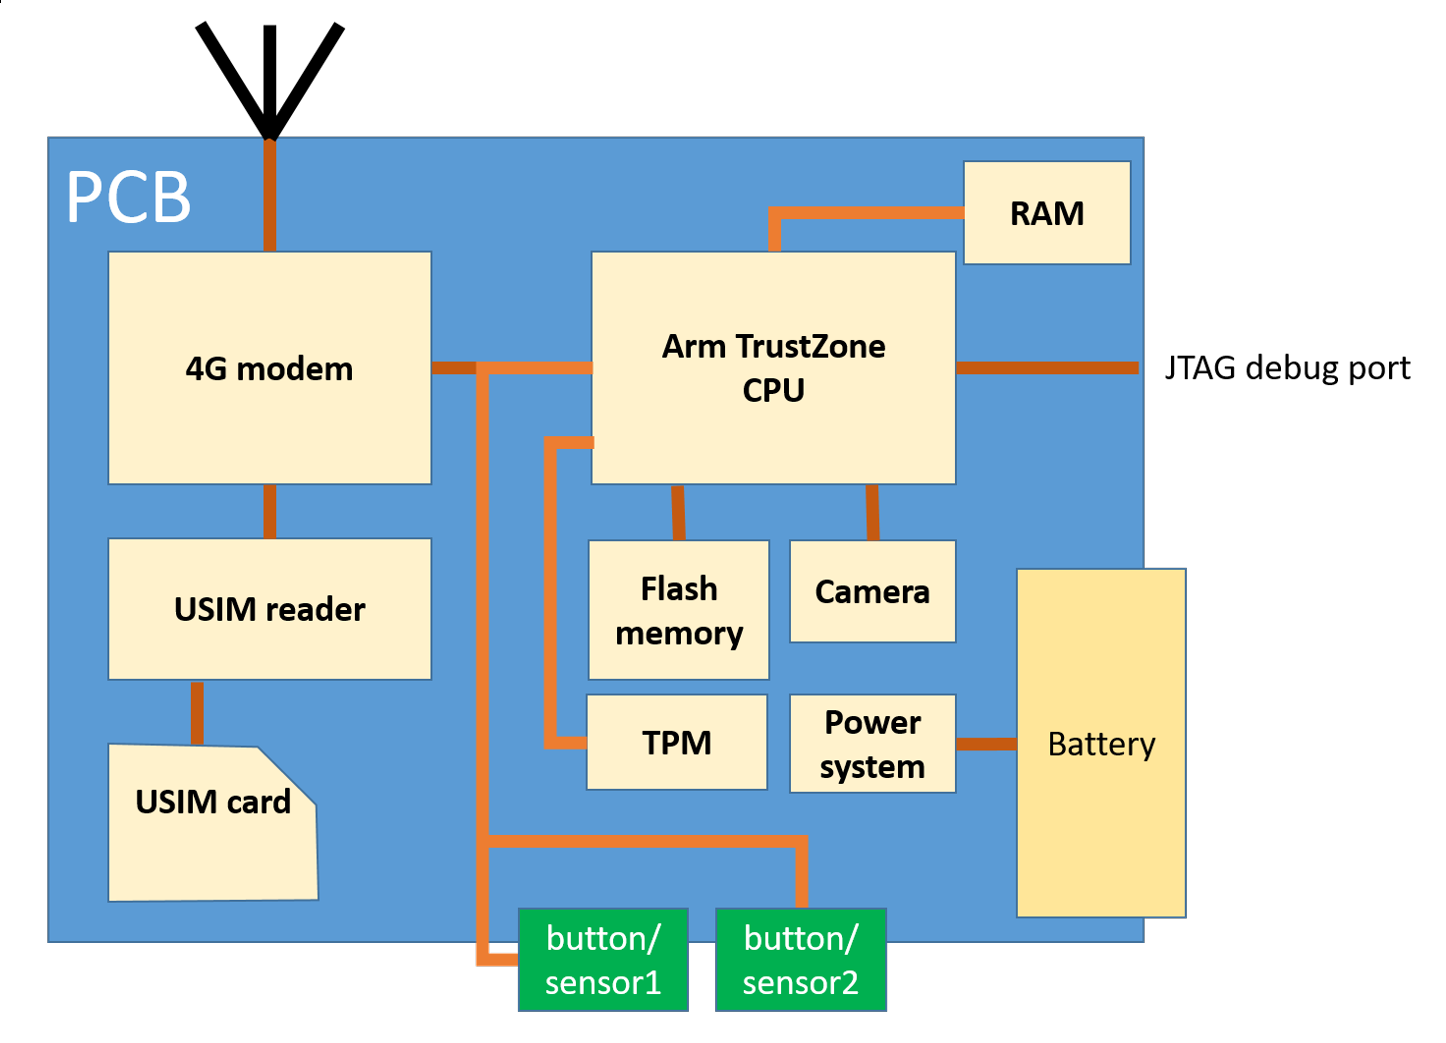
\includegraphics[width=0.5\textwidth]{input/pcb_camera.png}
      \end{figure}

      \subsubsection{Intended usage}

        The product is intended to be used as a perimeter security device for
        property owned by a company or the homes of private customers. The
        product is not intended to be used in high security environments such
        as banks or military installations.

      \subsubsection{Considered design requirements}

        % TODO: Write about all the requirements from the introduction.

      \subsubsection{Security assumptions}

         \begin{itemize}
           \assumption{LOCATION}{Mounting place}{
             The product is assumed to be mounted on the outer or inner walls of
             a building at a height that requires a small ladder to reach it.
           }
           \assumption{TIMELY\_MAINT}{Maintenance schedule followed}{
             It is assumed that the maintenance schedule is followed and that any
             defects or deteriorations outside of regular maintenance are
             reported as soon as they are detected.
		%TODO(?): What about user forgetting password? Handle through assumption 
		%of user with perfect memory here, or through specifying a software
		%'Forgot password?' functionality?
		\assumption{NO\_ADVERSARIAL}{No adversarial personnel}{
      	It is assumed that background checks on repair personnel are carried out.
    		}
           }
         \end{itemize}

  \section{Security architecture -- overview}

    \begin{figure}[H]
      \center
      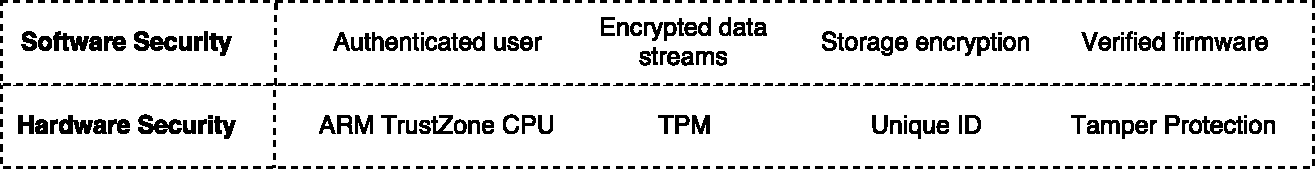
\includegraphics[width=0.9\textwidth]{input/security_layers.pdf}
      \caption{Schematic representation of hardware and software security layers.}
    \end{figure}

    \subsection{Hardware security layer}

      The hardware security layer of the platform consists of an ARM TrustZone
      CPU, a Trusted Platform Module for managing software security related
      artefacts, a static unique identifier created during the platform
      production and tamper detection to detect unauthorized attempts to
      access the hardware of the platform.

      \subsubsection{ARM TrustZone CPU}

        The ARM TrustZone CPU provides hardware level separation of trusted and
        untrusted region in the computational space. Using this feature in
        combination with a trusted OS and trusted boot a Trusted Execution
        Environment is created which can then act as a host to any trusted
        applications that will run on the platform.

        \begin{figure}[!h]
          \center
          % TODO: Make a draw.io copy of this picture.
          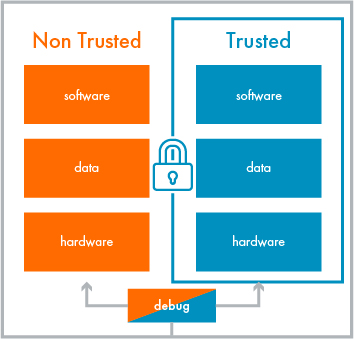
\includegraphics[width=0.4\textwidth]{input/arm_trust.jpg}
          \caption{ARM TrustZone security separation.}
        \end{figure}

        The CPU also features W xor X-protection by enabling its Nx-bit.
        Activating this feature reduces the attack-surface for code-injection
        attempts by making user-space memory either executable or modifiable,
        but not both. Since the platform includes management software for
        extracting operational information and remote configuration, this
        feature is of great interest.

      \subsubsection{Trusted Platform Module}

        The Trusted Platform Module (TPM) is a dedicated hardware component
        which main purpose is to provide a point-of-trust for handling security
        related software components and artifacts such as keys used for
        encryption, signing and identification. Beyond its storage
        capabilities the TPM also provides other higher-level functionality,
        such as verifying that the platform configuration and firmware has not
        been changed unknowingly (attestation), or making sure that some information
        is only available to the system at certain predefined states (sealing).

        By using the functionality made available by the TPM the platform is
        much better equipped to execute self-verification, storage and stream
        encryption and firmware- and configuration-updates in a cryptographically
        secure way.

      \subsubsection{Unique ID}

        Each camera platform PCB will have a unique 64-bit signature burned
        into it at production, ensuring that over 18 billion potential products
        can be uniquely identifiable.

      \subsubsection{Tamper detection}

        The camera housing is equipped with two tamper-switches; one that
        will detect if the camera is attached to a wall or not, and another
        switch that detects if the casing is open or closed.

    \subsection{Software security layer}

      The platform software security layer hinges mainly on the active usage of
      the onboard Trusted Platform Module (TPM) for tasks such as encryption,
      attestation and authentication. The CPU has complementary
      security-features that, while not possible to use in the software layer
      directly, enables a more trust-based boot and execution model with a
      reduced attack-surface for commonly used exploit-types, which reduce the
      impact of potential software-bugs.

      \subsubsection{User authentication}

        It is imperative that the audio and video data produced by the
        platform, together with any configuration and user information stored
        on the device is only made available to trusted users of the system,
        and out of reach to anyone gaining unauthorized access to the system.
        To ensure that this is the case, the data mentioned above will be
        encrypted together with using a username and password combination to
        issue a challenge-response when access is requested.

        The system will recognise three types of users; regular users,
        maintenance users and a root user. The regular users will only have
        access to their own data and configuration options related to the user
        experience of using the platform. Maintenance users will have access to
        additional configurations and diagnostic information related to the
        upkeep and day-to-day operations of the platform. The root user will
        have access to all configuration options and diagnostic data  available
        on the platform together with the ability to create or remove any of
        the other types of users from the system.

        It is worth to point out that the root user will not have default
        access to any of the local users encrypted data without knowing their
        specific password.

      \subsubsection{Encrypted data streams}

        Since the main transmission of data and general communication with the
        platform occurs wirelessly through the use of a 4G modem, the stream
        needs to be encrypted and verifiable in order to not be readable or
        modifiable in transit. This is achieved by utilizing the Secure
        Real-time Transport Protocol (SRTP), which provides authentication,
        integrity and reply protection, for both data transfer and
        communication to and from the platform.

      \subsubsection{Storage encryption}

        In order to ensure that there is not sensitive data to access on
        unauthorized access, especially physical removal of storage, any
        non-trivial configuration data together with all diagnostic and
        user-data is encrypted using 256-bit AES. The symmetric key will be
        derived from the combination of a TPM storage key together with the
        username and a hash of the specific challenge-response result for the
        given username and password combination.
        %TODO: Unsure if we should involve the TPM storage key, user has to
        %have a TPM to decrypt any transmitted blobs. Maybe unnecessary since
        %it transmits through SRTP? R: Yeah, sounds fair. 

      \subsubsection{Verified firmware}

        In order to ensure that the platform can be seen as trusted, it has to
        be able to ensure that it is running verified firmware. This is
        accomplished in two steps; first the platform should not be able to run
        any arbitrary code, only code that has been specifically verified to be
        trusted. Secondly, the platform should be able to detect any
        non-sanctioned modifications to its software configuration and report
        that these have happened and either run with reduced capabilities or
        not at all.

        Both of these steps are accomplished via the usage of the onboard TPM.
        By using another TPM to sign the firmware, the platform TPM, with
        the correct keys migrated, can verify that the firmware it is asked to
        load is trusted, or refuse otherwise. For the second step, the software
        configuration can be verified by using the TPM's sealing capabilities.
        If the current software and configuration does not generate a hash
        value that matches a stored one, vital security resources such as
        decryption and session keys can be withheld, prompting the system to
        signal that something is wrong.

    \begin{itemize}
      \item User, connected to: '4G modem'
      \begin{itemize}
        \item TPM
      \end{itemize}
      \item Maintenance Person, connected to: \{'4G modem' for remote management, 'JTAG debug port' for close management\}
      \begin{itemize}
        \item TPM
      \end{itemize}
      \item Power supply, connected to: 'Battery'
      \item Repair Person, connected to: all components of camera %state this, don't draw it..
    \end{itemize}
    \textbf{Changes to PCB picture}
    \begin{itemize}
      \item Change 'button/sensor1' to 'Tamper switch'
      \item Remove 'button/sensor2'
      \item Add 'Burnt-in Master Key', connected to: TPM(?) %R@S: where is this 'burnt in'?
      \item Add text 'SRTP', connected to: 4G modem antenna
      \item ? Add text 'Encryption of video data', connected to path between CPU and Flash memory ? % perhaps too detailed
      %\item Add `Key Blobs (TPM)', in Flash
    \end{itemize}
    \textbf{TPM}
    \begin{itemize} %perhaps not have keys at all
      \item EK
      \item SRK
      \item AIK
    \end{itemize}

    \subsubsection{Life cycle of TOE}
    \begin{itemize}
      \item 'Production', connected to: 'User operation'
      \item 'User operation', conn to: \{'Service/repair', 'Maintenance'\}
      \item 'Maintenance', conn to: 'User operation'
      \item 'Service/repair', conn to: \{'User operation', 'Decommission'\}
      \item 'Decommission'
    \end{itemize}

	\subsubsection{Assets}

      The product contains two types of valuable assets; physical and
      non-physical. Among the product hardware, the TPM and flash memory
      are of special interest from a security perspective since these house
      configuration data, stored video recordings and security related
      information. The non-physical assets consist of security keys used for
      encrypting communication, video-transmission and storage, together with
      the video recordings themselves and possible sensitive configuration
      information.

 \subsubsection{Security objectives for the TOE}
	\begin{itemize}
		\objective{TPM\_KEY\_STRG}{Storage of keys in camera}{
      The storage of internal keys of camera should be done in the TPM.
    }
		\objective{TRUSTZONE\_NX}{Nx enabled in ARM CPU}{
      The ARM Trustzone CPU should have Nx bit enabled.
    }
		\objective{DECOMM}{Easy erasure of data}{
      When the TOE is decommissioned, it should be easy for the user to make
      stored user information and data stored unreadable (or wiped).
    }
		\objective{ID}{Strong identity}{
      The camera should have a unique, cryptographically strong, identity that
      is burned into the PCB during camera manufacturing.
    }
		\objective{NO\_TAMPER}{Detect tampering}{
      The TOE should have two tamper switches: one on backside of housing in order to
      detect if pulled off of wall, one inside housing behind battery hatch in order to detect if opened.
    }
		\objective{PWR\_OUT}{Notify if lost power}{
      A notification should be sent to User and Maintenance Personnel if connection to power source is cut off.
    }
		\objective{ATTEST}{Attestation used for remote}{
      When a Maintenance Person is to update firmware, attestation should be
      carried out with the help of the TPMs in MP's computer and the TOE.
    }
		 \objective{SECURE\_COMMS}{Secure communictions}{
             The TOE should have a correct configuration that
             enables a fully encrypted and authenticated SRTP stream to be used
             for data transfer, and also use it.
           }
		\objective{TWO\_WAYS\_PROT}{Two-ways protection}{
		 Forwards and backwards protection by reapplying the key derivation
		function for the SRTP connection.	
    }
	\end{itemize}
        % TODO: Expand with more security features.
        % TODO: Determine the X in X-bt encrypted RSTP stream.
        %The product features secure video streaming capabilities through a
        %X-bit encrypted SRTP stream with fully encrypted data storage.

        % Split it into hardware/software?

%        Forwards and backwards protection by reapplying the key derivation
%		function for the SRTP connection.

  %\subsubsection{Security Objectives for the Operational Environment}
	%\begin{itemize}
		%\objenv{NO\_ADVERSARIAL}{No adversarial personnel}{
     % It is assumed that background checks on repair personnel are carried out.
    %} % R: maybe not have this, but could mitigate T_ADVERSARIAL. Otherwise, an
      % example of OpEnv-obj
	%\end{itemize}

  \section{Security problem definition}

    \subsection{Security solutions}

      %Short security evaluation of the design that explained the used security
      %measures and the motivation behind them. Should include a list of all
      %threats and security issues that are deemed applicable to the system,
      %together with any threats that were deemed a non-issue.

      %This section contains a table where the problems are listed on the y-axis
      %against the solutions on the x-axis where a 'X' marks with solution
      %protects against which threat.

 \subsubsection{Threat agents}

      The following attack vectors are deemed relevant for the product.
      Physical attacks in order to disable and dismantle product by
      unauthorized individual inside perimeter. Extracting non-physical
      assets ill-intentioned maintenance personnel, analyzing data in
      traffic or by unauthorized network access.

    \subsubsection{Threats}
      \begin{itemize}[label={}]
        \threat{PHYSICAL}{Physical Access} {
          An attacker can physically access the camera. This can result in
          destruction of camera in pure vandalizing, removal of camera from
          premises opening up for other threats (T.FLASHMEM\_INTEGRITY and T.LOST\_ASSET), covering camera
          with other physical object or smearing something on camera
          housing/lens rendering recorded video useless.
        }
        \threat{NETWORK}{Network attack} {
          Since the camera is outfitted with a 4G subsystem, attacks relevant for
          such a system are relevant here. }
        \threat{MISMANAGE}{Incompetent personnel} {
          There is a risk that the persons managing and servicing the camera do
          not have the skills required, which can result in password being
          leaked, physical components of camera damaged, camera not mounted on
          wall correctly etc.
        }
        \threat{ADVERSARIAL}{Adversarial repair personnel}{ 
          The repair personnel may be dishonest and try to access the video
          files, the keys, may try to inject code or access internal memory of
          camera.
        }
        \threat{PERSISTENT}{Persistent presence}{
          If the (remote) management system is flawed an attacker could, access camera through the
          management interface at their convenience.
        }
        \threat{LOST\_ASSET}{Camera/key is lost}{
          An attacker either physically makes off with a camera or gets hold of
          a crypto key.
        }
        \threat{MANAGEMENT\_TESTING}{Faulty management software}{
          If bugs exist in the (remote) management system, that would allow an attacker to
          insert executable foreign code.
        }
        \threat{SIGNED\_FIRMWARE}{Running unauthorized firmware}{
          An attacker could load unauthorized firmware.
        }
        \threat{SRTP\_RECV}{Loading non-matching SRTP keys}{
          An attacker could load SRTP keys for an incorrect receiver.
        }
        \threat{FLASHMEM\_INTEGRITY}{Flashing faulty code/config}{
          Include safeguards concerning removing flash memory and loading it
          with altered configurations or code.
        }
        \threat{JTAG\_ABUSE}{Unauthorized access through JTAG}{
          Secure JTAG debug interface against misuse. %Check article about JTAG interface attacking from first part of course.
        }

        % TODO: Do we want this?
        %\threat{DESOLDER}{Dismantling/modifying physical components}{
          %From first part of course, attack where microprocessor is removed
          %and is either probed or re-soldered (BGA) in order to access memory.
          %Defense against this dark art? Check article again. Note: perhaps
          %part of 'flash memory' entry above in this list. Or T.LOST\_ASSET.
        %}
      \end{itemize}

      \subsubsection{Rationale}
	%Here, could do tables as in https://www.commoncriteriaportal.org/files/epfiles/ST-FFHDD.pdf

      \subsubsection{Coverage}
        
\begin{tabular}{| l | c | c | c | c | c | c | c | c | c | c | c | c | c |}
 \cline{2-14}
 \multicolumn{1}{c|}{}  & \rotatebox{90}{O.TPM\_KEY\_STRG} & \rotatebox{90}{O.TRUSTZONE\_NX} & \rotatebox{90}{O.DECOMM} & \rotatebox{90}{O.ID} & \rotatebox{90}{O.NO\_TAMPER} & \rotatebox{90}{O.PWR\_OUT} & \rotatebox{90}{O.ATTEST} & \rotatebox{90}{O.SECURE\_COMMS} & \rotatebox{90}{O.TWO\_WAY\_PROT} & \rotatebox{90}{O.ENC\_DATA} & \rotatebox{90}{O.TPM\_SEAL} & \rotatebox{90}{A.LOCATION} & \rotatebox{90}{A.NO\_ADVERSARIAL} \\
\hline
T.PHYSICAL &   &   &   &   & X &   &   &   &   &   &   & X &   \\
\hline
T.NETWORK &   &   &   &   &   &   &   & X & X &   &   &   &   \\
\hline
T.MISMANAGE &   &   &   &   &   &   &   &   &   &   & X &   & X \\
\hline
T.ADVERSARIAL &   &   &   &   &   &   &   &   &   &   & X &   & X \\
\hline
T.PERSISTENT &   &   &   &   &   &   &   &   &   &   &   &   &   \\
\hline
T.LOST\_ASSET &   &   &   & X &   &   &   &   &   & X & X &   &   \\
\hline
T.MNG\_TEST &   &   &   &   &   &   &   &   &   &   &   &   &   \\
\hline
T.SIGNED\_FW & X &   &   &   &   &   &   &   &   &   &   &   &   \\
\hline
T.SRTP\_RECV &   &   &   &   &   &   &   &   &   &   &   &   &   \\
\hline
T.FLASH\_INTG &   &   &   &   &   &   &   &   &   &   &   &   &   \\
\hline
T.JTAG\_ABUSE &   &   &   &   &   &   &   &   &   & X &   & X &   \\
\hline
\end{tabular}



  \section{Peer reviews}

  \section{Improvement sheet}

  \begin{thebibliography}{9}
	\bibitem{stwiki} \textit{Security Target - Wikipedia} \url{https://en.wikipedia.org/wiki/Security_Target}
  \end{thebibliography}

\end{document}
